\documentclass[conference]{IEEEtran}

\usepackage[]{graphicx}    % We use this package in this document
\usepackage{amsmath}
\usepackage{mathtools}
\usepackage{subfiles}
\usepackage{amssymb}
\usepackage{hyperref}
\usepackage{algorithm}
% \usepackage{algorithmic}
\usepackage{tikz,tikz-3dplot}
\usepackage{pgfplots}
\usepackage{subcaption}
\usepackage{arevmath}     % For math symbols
\usepackage[noend]{algpseudocode}
\usepackage[margin=1.5in]{geometry}    % For margin alignment
\usepackage[english]{babel}
\usepackage[utf8]{inputenc}


\newcommand{\ignore}[1]{}  % {} empty inside = %% comment
\graphicspath{ {./pics/} }

\ifCLASSINFOpdf
\else
\fi

\hyphenation{op-tical net-works semi-conduc-tor}


\begin{document}

\title{Heterogenous Autonomous Robotic Exploration (HARE)}

\author{Jackson~Parker, Allen Spain, Caleb Adams}

% The paper headers
\markboth{IEEE JOURNAL XXXX, VOL. XX, NO. XX, MONTH 20XX}%
{Shell \MakeLowercase{\textit{et al.}}: Bare Demo of IEEEtran.cls for IEEE Journals}

% \markboth{IEEE JOURNAL OF SELECTED TOPICS IN APPLIED EARTH OBSERVATIONS AND REMOTE SENSING, VOL. XX, NO. XX, MONTH 20XX}



% If you want to put a publisher's ID mark on the page you can do it like
% this:
%\IEEEpubid{0000--0000/00\$00.00~\copyright~2015 IEEE}
% Remember, if you use this you must call \IEEEpubidadjcol in the second
% column for its text to clear the IEEEpubid mark.



% use for special paper notices
%\IEEEspecialpapernotice{(Invited Paper)}




% make the title area
\maketitle

% As a general rule, do not put math, special symbols or citations
% in the abstract or keywords.
\begin{abstract}
  The purpose of this research is to prove that subtask division can be accomplished based on knowledge of robot capabilities. To prove this, we are developing an exploration system in which robots with different hardware and capabilities will work together to accurately explore and map a complex region of space. Through the definition of individual attributes and the sharing of those attributes, each robot will search and map regions of space that it is capable of maneuvering. Instead of simple binary mapping of the region, 1 = free space and 0 = obstacle, each robot will mark the region that it has explored and can maneuver through this a specific identifier. This gives the region itself a bit of information as well as allows other robots to help determine if they are capable of maneuvering as well.
  Once a robot comes to an obstacle or region that it cannot maneuver around, it will evaluate which team members are capable of doing so and mark that space for the capable robots to explore. Due to time limitations on this project, instead of relying on complex perceptive capabilities to evaluate which robots could explore that region, the utilization of object id which can be surveyed by the robots sensors to compare its own attributes with the attributes necessary for exploration.
\end{abstract}

% Note that keywords are not normally used for peerreview papers.
\begin{IEEEkeywords}
IEEE, IEEEtran, journal, \LaTeX, paper, template, Multi-Robot Systems, exploration, autonmous mobile robots, heterogenous, BFS, behavior trees
\end{IEEEkeywords}


\IEEEpeerreviewmaketitle

\begin{figure}[H]
  \centering
    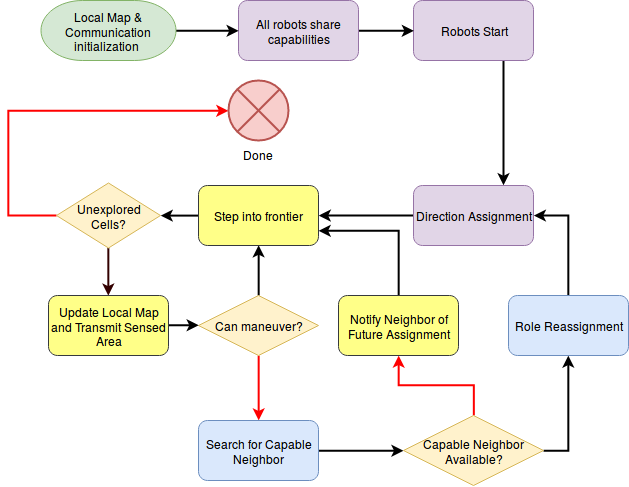
\includegraphics[width=0.5\textwidth]{HARE}
  \caption{High level block diagram for HARE}
  \label{fig:something3}
\end{figure}

%%%%%%%%%%%%%%%%%%%%%%%%%%%%%%%%%%%%%%
\section{Introduction}
%%%%%%%%%%%%%%%%%%%%%%%%%%%%%%%%%%%%%%
\subfile{tex/intro}

%%%%%%%%%%%%%%%%%%%%%%%%%%%%%%%%%%%%%%%%%%%
\section{Methodology}
%%%%%%%%%%%%%%%%%%%%%%%%%%%%%%%%%%%%%%%%%%%
\subfile{tex/methodology} %  <-- might be best to keep the example and remake some subfiles

%%%%%%%%%%%%%%%%%%%%%%%%%%%%%%%%%%%%%%%%%%%
\section{Results}
%%%%%%%%%%%%%%%%%%%%%%%%%%%%%%%%%%%%%%%%%%%
\subfile{tex/results} %  <-- might be best to keep the example and remake some subfiles

%%%%%%%%%%%%%%%%%%%%%%%%%%%%%%%%%%%%%%%%%%%
\section{Conclusion}
%%%%%%%%%%%%%%%%%%%%%%%%%%%%%%%%%%%%%%%%%%%
\subfile{tex/conclusion} %  <-- might be best to keep the example and remake some subfiles


% use section* for acknowledgment
\subfile{tex/appendix}
% \section*{Acknowledgment}

\ifCLASSOPTIONcaptionsoff
  \newpage
\fi



\bibliographystyle{IEEEtran}
% \bibliography{sources}
\bibliography{IEEEabrv,sources} % ftp://tug.ctan.org/pub/tex-archive/macros/latex/contrib/IEEEtran/bibtex/IEEEtran_bst_HOWTO.pdf


% insert where needed to balance the two columns on the last page with
% biographies
%\newpage

\begin{IEEEbiography}[{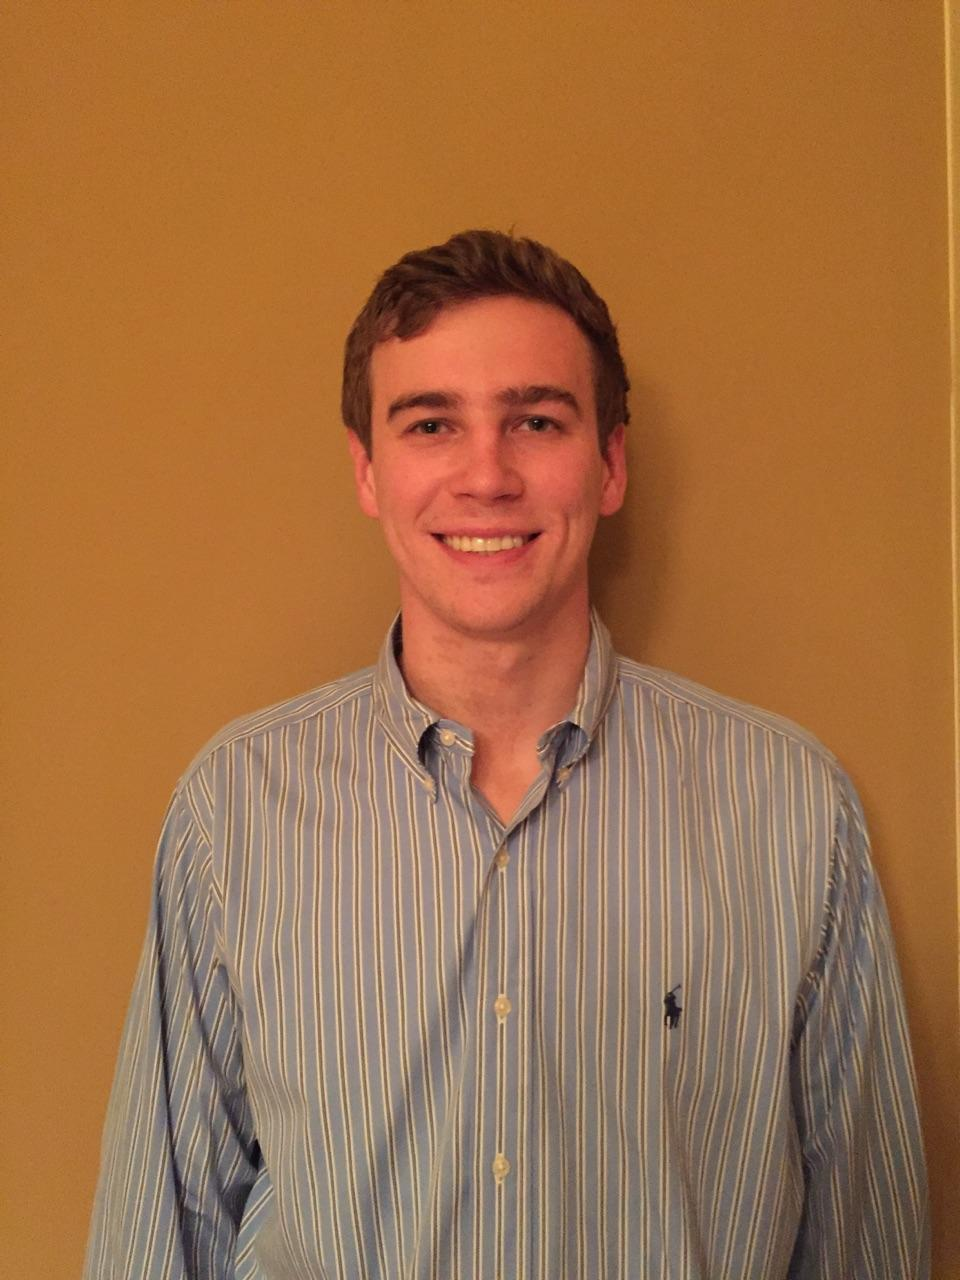
\includegraphics[width=1in,height=1.25in,clip,keepaspectratio]{pics/jackson_parker}}]{Jackson Parker}
I work in the small satellite research lab as a systems engineer.
\end{IEEEbiography}


\begin{IEEEbiography}[{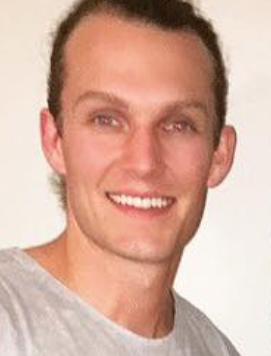
\includegraphics[width=1in,height=1.25in,clip,keepaspectratio]{pics/allen}}]{Allen Spain}
Lead Hardware Engineer Small Satellite Research Laboratory.
\end{IEEEbiography}




\end{document}
